\documentclass[12pt]{article}
\usepackage[spanish]{babel}
\usepackage{natbib}
\usepackage{url}
\usepackage[utf8x]{inputenc}
\usepackage{amsmath}
\usepackage{float}
\usepackage{subfig}
\usepackage{graphicx}
\graphicspath{{images/}}
\usepackage{parskip}
\usepackage{fancyhdr}
\usepackage{vmargin}
\usepackage{mathtools}
\usepackage{amssymb} 



\title{Actividad \#7:El Espacio Fase}							
\author{\Large Jesùs Valenzuela Nieblas\\}											
\date{\today} 

\makeatletter
\let\thetitle\@title
\let\theauthor\@author
\let\thedate\@date										
\makeatother

\pagestyle{fancy}

\lhead{\thetitle}
\cfoot{\thepage}
\rhead{}
\begin{document}

%%%%%%%%%%%%%%%%%%%%%%%%%%%%%%%%%%%%%%%%%%%%%%%%%%%%%%%%%%%%%%%%%%%%%%%%%%%%%%%%%%%%%%%%%

\begin{titlepage}
	\centering
    \vspace*{.5cm}
     
\includegraphics[scale = 0.7]{logo}\\	% University Logo
    \textsc{\Large Universidad de Sonora}\\[1.0 cm]	% University Name
	\textsc{\Large División de Ciencias Exactas y Naturales}\\[.50 cm]
  	\textsc{\Large Licenciatura en Fìsica}\\[.5 cm]
  \textsc{\large Fìsica Computacional 1}\\[1.5 cm]				% Course Name
	
	{ \huge \bfseries \thetitle}\\

    \vspace*{3 cm}
	\begin{minipage}{\textwidth}
    \centering
    \theauthor
	\end{minipage}\\[3 cm]
	
 
	\vfill
	
\end{titlepage}

%%%%%%%%%%%%%%%%%%%%%%%%%%%%%%%%%%%%%%%%%%%%%%%%%%%%%%%%%%%%%%%%%%%%%%%%%%%%%%%%%%%%%%%%%

\section{Introducciòn}
En mecánica clásica, el espacio fásico, espacio de fases o diagrama de fases es una construcción matemática que permite representar el conjunto de posiciones y momentos conjugados de un sistema de partículas. Más técnicamente, el espacio de fases es una variedad diferenciable de dimensión par, tal que las coordenadas de cada punto representan tanto las posiciones generalizadas como sus momentos conjugados correspondientes. Es decir, cada punto del espacio fásico representa un estado del sistema físico. Ese estado físico vendrá caracterizado por la posición de cada una de las partículas y sus respectivos momentos.

El formalismo del espacio fásico se emplea en el contexto de la mecánica lagrangiana y la mecánica hamiltoniana. Usualmente se designa el espacio fásico o una parte de él por $\Gamma$ (gamma mayúscula). Físicamente cada punto del espacio fásico representa un posible estado del sistema mecánico.

En física estadística se usan distribuciones de probabilidad definidas sobre el espacio fásico. Partiendo de cierto subconjunto de las distribuciones de probabilidad de un espacio fásico puede construirse una estructura de espacio de Hilbert. Estos espacios de Hilbert de un sistema clásico son la base para los espacios de Hilbert que aparecen en mecánica cuántica.
\section{Actividad}

El còdigo utilizado es el siguiente:
\begin{verbatim}
import numpy as np
import matplotlib.pyplot as plt
from scipy.integrate import odeint

def pend(y, t, b, c):
        theta, omega = y
        dydt = (omega, -b*omega - c*np.sin(theta))
        return dydt
        
b = 0           
g= 9.8           
l=1              
c=g/l
t = np.linspace(0.0,20,500)  

X_f1 =np.array([-90.0*np.pi,20])
X_f2 =np.array([-2.0*np.pi,0.0]) 


values1 =np.linspace(-1,1,45)                
values2 =np.linspace(-1,1,90)                
vcolors1 = plt.cm.flag(np.linspace(.7, .2, len(values1))) 
vcolors2 = plt.cm.gist_ncar(np.linspace(0.4, 0.8, len(values2)))  

plt.figure(2)


#Trayectorias de arriba
for v1, col1 in zip(values1, vcolors1):
    y1 = v1 * X_f1                                
    x1 = odeint(pend, y1, t, args=(b,c))         
    plt.plot( x1[:,0], x1[:,1], lw=1.5*v1, color=col1 )

#Trayectorias del centro                             
for v2, col2 in zip(values2, vcolors2):
    y2 = v2 * X_f2                                 
    x2 = odeint(pend, y2, t, args=(b,c))           
    plt.plot( x2[:,0], x2[:,1], lw=1.5*v2, color=col2 )


#Para graficar
plt.title('Espacio Fase')
plt.xlabel('Angulo')
plt.ylabel('Velocidad Angular')
plt.grid()
plt.xlim(-3.0*np.pi,3.0*np.pi)
plt.ylim(-15,15)


plt.show()
\end{verbatim}
\subsection{Gráfica Generada}
\begin{figure}[H]
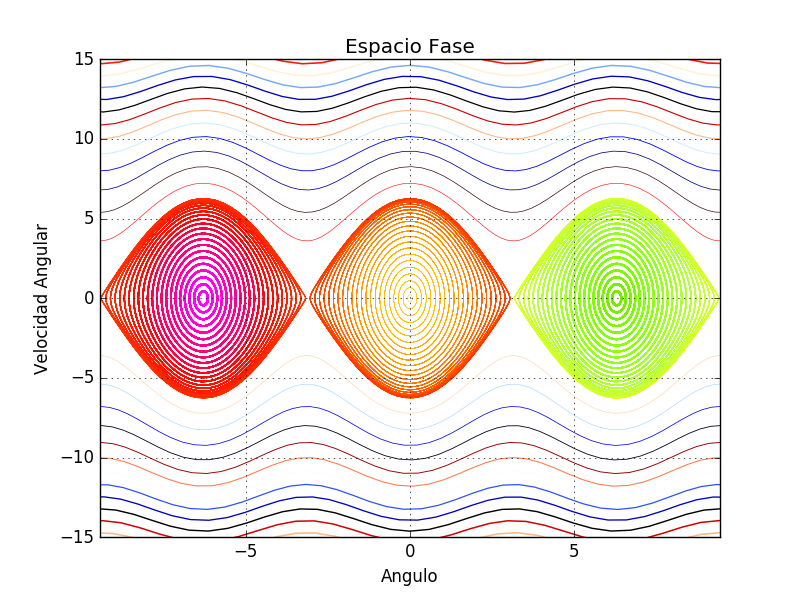
\includegraphics[scale=.8]{efase}
\end{figure}


\end{document}
